\documentclass[dwyatte_dissertation.tex]{subfiles} 
\begin{document}

\chapter{Effects of spatial and temporal prediction during novel object learning}

\section{Introduction}
TODO

\section{Methods}

\subsection{Participants}
A total of 62 students from the University of Colorado Boulder participated in the experiment (ages 18-22, mean=19.11 years; 30 male, 32 female). All participants reported normal or corrected-to-normal vision and received course credit as	compensation for their participation. Informed consent was obtained from each participant prior to the experiment in accordance with Institutional Review Board policy at the University of Colorado.

\subsection{Stimuli}
Novel ``paper clip'' objects were used as stimuli (see Chapter \ref{chap:pleast} Methods). A total of eight objects were used -- four as targets and four as distractors. The four target objects were also used in the experiment described in Chapter \ref{chap:pleast}. Target and distractor objects were paired together for the purposes of the experiment. All objects are shown in Figure \ref{fig:paperclip}.

% paperclip targets fig
\begin{figure}[h!]
\textbf{A} \\
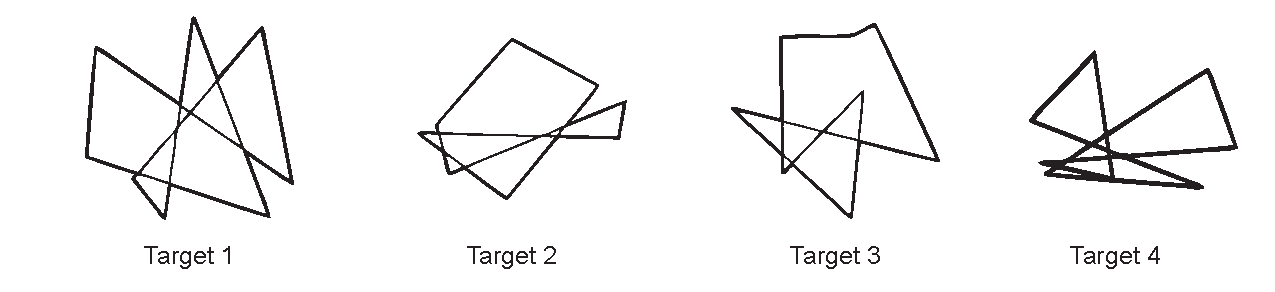
\includegraphics[width=160mm]{figs/bpleast/paperclip_targets.pdf} \\
\textbf{B} \\
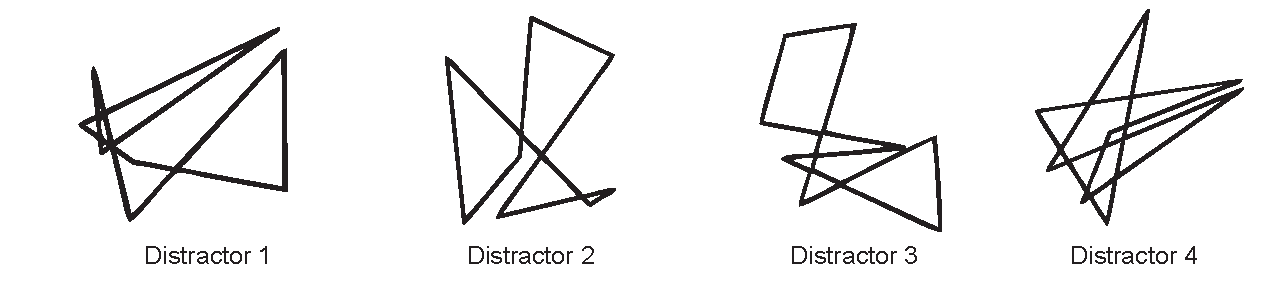
\includegraphics[width=160mm]{figs/bpleast/paperclip_distractors.pdf} \\
\caption{Novel ``paper clip'' objects}{Four target (\textbf{A}) and four distractor object pairs (\textbf{B}) used in the experiment. See Chapter \ref{chap:pleast} Methods for additional information.}
\label{fig:paperclip}
\end{figure}

\subsection{Procedure}
The experiment was divided into 16 blocks, each containing a training period followed by a series of test trials (Figure \ref{fig:task}). During the training period of a given block, participants observed one of the target objects rotate about its y-axis. The object either rotated coherently (i.e., spatially predictable, S+ conditions) or in a random manner (S- conditions). Coherent rotation was composed of adjacent views spaced 12 degrees apart. The object made four complete rotations during the study period. All views of the object were still presented four times each in the random case. The presentation rate during the study period was either 10 Hz with a 50 ms on time and 50 ms off time (i.e., temporally predictable, T+ conditions) or variable with a 50 ms on time and off times ranging from 16.67-400 ms (T- conditions). 

The S+/- and T+/- conditions were crossed and each of the target-distractor object pairs was assigned to one of the four conditions. These assignments were approximately counterbalanced across subjects (Assignment 1: \textit{N}=15; Assignment 2: \textit{N}=17; Assignment 3: \textit{N}=15; Assignment 4: \textit{N}=15). Each block condition with its target-distractor pairing was repeated for four blocks during the experiment (block ordering randomized).

During each block, subjects were instructed to study the target object during the training period and then complete a series of 30 test trials. On each test trial, either the target object or its paired distractor was presented. Subjects were instructed to respond ``same'' if they believed the object depicted the trained target object or ``different'' if they believed it depicted the distractor object. Half of the test trials contained 15 views of the target object spaced 24 degrees apart, and the other half contained 15 views of the distractor, also spaced 24 degrees apart. Test trials were shown in a random order and feedback was withheld to prevent participants from changing their response criteria over the course of a block. 

The experiment was displayed on an LCD monitor with a native resolution of 1280x1024 operating at 60 Hz using the Psychophysics Toolbox Version 3 \cite{Brainard97,Pelli97}. All stimuli were presented on an isoluminant 50\% gray background and subtended approximately 5 degrees of visual angle. Test trials began with a fixation cross (200 ms) followed by a blank (400 ms) followed by the probe stimulus (100 ms). Participants were required to respond within 2000 ms. Subsquent test trials were separated by a variable intertrial interval of 1000-1400 ms.

The experiment began with a practice block to ensure that participants understood the task. The training period during the practice block was always spatially and temporally predictable and used a reserved target object and distractor that were not further used in any of the experimental blocks. During the practice test trials, subjects received feedback after responding according to whether they were correct or incorrect. After completing the practice block, subjects were informed that future training periods could be presented in spatially and/or temporally unpredictable manners.

% paperclip targets fig
\begin{figure}[h!]
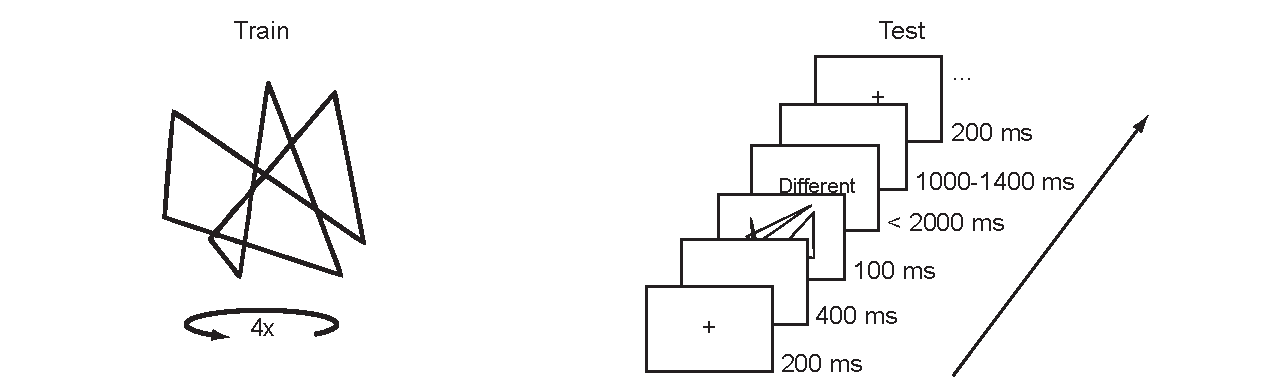
\includegraphics[width=160mm]{figs/bpleast/paperclip_task.pdf} \\
\caption{Experimental procedure}{}
\label{fig:paperclip}
\end{figure}

\section{Results}

\section{Discussion}

\bibliographystyle{apa}
\bibliography{ccnlab}
\end{document}